\section{Statistische Analyse der Ergebnisse}
\label{sec:chi}

Im vorherigen Kapitel wurde die Übereinstimmung der Daten mit den Simulationen bereits qualitativ durchgeführt.
Um nun die Übereinstimmung quantitativ zu bestimmen, wird ein $\Chi^2$-Test durchgeführt.
Dieser $\Chi^2$-Test ist ein statistisches Maß um die Abweichung zwischen einer beobachteten und erwarteten Verteilung zu bestimmen.
Die erwartete Verteilung entspricht dabei den Monte-Carlo Simulationen, also der Untergrundverteilungen plus einer spezifischen Massenhypothese des $Z^\prime$.
Die beobachtete Verteilung entspricht den gemessenen Daten.
Die Prüfgröße $\Chi^2$ berechnet sich dann durch

\begin{equation}
  \Chi^2 = \sum_{j=1}^m \frac{(N_j - n_{0j})^2}{n_{0j}}
\end{equation}

und gibt die Größe der Abweichung in jedem Bin der Verteilung an.
Dabei ist $N_j$ die beobachtete und $n_{0j}$ die erwartete Häufigkeit.
Dies wird auf dem Datensample \texttt{data.mu.2.root} für die Diskriminante, also der invarianten Masse des Systems durchgeführt.
Ist die Nullhypothese, dass es ein $Z^\prime$ gibt, wahr, so muss der Unterschied zwischen $N_j$ und $n_{0j}$ sehr gering sein.
Das Konfidenzlevel berechnet sich aus $p = 1 - \alpha$, wobei $\alpha$ die Signifikanz des Tests ist.
Damit eine Hypothese angenommen wird, muss $\Chi^2 < \Chi^2_{1-\alpha}$ gelten.
Das Konfidenzlevel wird durch das Paket \texttt{TMath} von \texttt{root} berechnet und ist von der Anzahl an Freiheitsgraden, bzw. Bins abhängig.
Da keine Hinweise auf ein mögliches $Z^\prime$ gefunden wurden, kann in einem nächsten Schritt eine obere Ausschlussgrenze im $\SI{95}{\percent}$ Konfidenzintervall für die verschiedenen $Z^\prime$-Massenhypothesen gefunden werden.
Um die Gewichte der einzelnen Hypothesen zu berücksichtigen wird ein scaler genutzt, der die Gewichte entsprechend skaliert bis das $\SI{95}{\percent}$ Konfidenzintervall erreicht wurde.
Diese Ergebnisse sind in Tabelle \ref{tab:chi2} dargestellt.
Wie zuvor festgestellt, kann keine der Massenhypothesen bestätigt werden.
Sie alle erfüllen die geforderte Signifkinaz nicht.

\begin{table}
  \centering
  \caption{Die berechneten Parameter des $\Chi^2$-Tests für eine reine Untergrundverteilung und den verschiedenen $Z^\prime$-Massenhypothesen. Für die Massenhypothesen wurde außerdem die erwartete obere Ausschlussgrenze des Wirkungsquerschnittes im $\SI{95}{\percent}$ Konfidenzintervall berechnet.}
  \label{tab:chi2}
  \begin{tabular}{c|ccccc}
    \toprule
    Process & Freiheitsgrade & Konfidenzlevel & $\Chi^2$ & scaler & $\sigma / \si{\pico\barn}$ \\
    Reiner Untergrund & 11 & 0.9162 & 5.29 & - & - \\
    $Z^\prime (400)$  & 11 & 0.0209 & - & 0.3 & 33 \\
    $Z^\prime (500)$  & 11 & 0.0008 & - & 0.2 & 16.4 \\
    $Z^\prime (750)$  & 11 & 0.012 & - & 0.2 & 4 \\
    $Z^\prime (1000)$ & 11 & 0.0461 & - & 0.4 & 2.2 \\
    $Z^\prime (1250)$ & 11 & 0.0257 & - & 0.9 & 1.71 \\
    $Z^\prime (1500)$ & 11 & 0.0429 & - & 1.9 & 1.58 \\
    $Z^\prime (1750)$ & 11 & 0.0470 & - & 5.5 & 1.65 \\
    $Z^\prime (2000)$ & 11 & 0.0483 & - & 12.5 & 1.75 \\
    $Z^\prime (2250)$ & 11 & 0.0493 & - & 25.1 & 1.68 \\
    $Z^\prime (2500)$ & 11 & 0.0497 & - & 53.2 & 1.86 \\
    $Z^\prime (3000)$ & 11 & 0.489 & - & 213.4 & 2.56 \\
    \midrule
    \bottomrule
  \end{tabular}
\end{table}

Abschließend werden die so berechneten erwarteten oberen Ausschlussgrenzen der Wirkungsquerschnitte im $\SI{95}{\percent}$ Konfidenzintervall der unterschiedlichen $Z^\prime$-Massenhypothesen gegen ihre Masse aufgetragen.
Dies wird mit den erwarteten Wirkungsquerschnitten verglichen.
Das ist in Abbildung \ref{fig:limit} dargestellt.
Aus diesen Plots ist erkennbar, dass nur Massen bis $\SI{1250}{\giga\electronvolt}$ erlaubt sind.
Allerdings wurden in den in Kapitel \ref{sec:aufgabe6} angefertigten stacked Plots keine entsprechenden Hinweise gefunden.
Die höheren Massen können ausgeschlossen werden, da die Daten ansonsten nicht zu dem simulierten Untergrund passen würden.

\begin{figure}
    \centering
    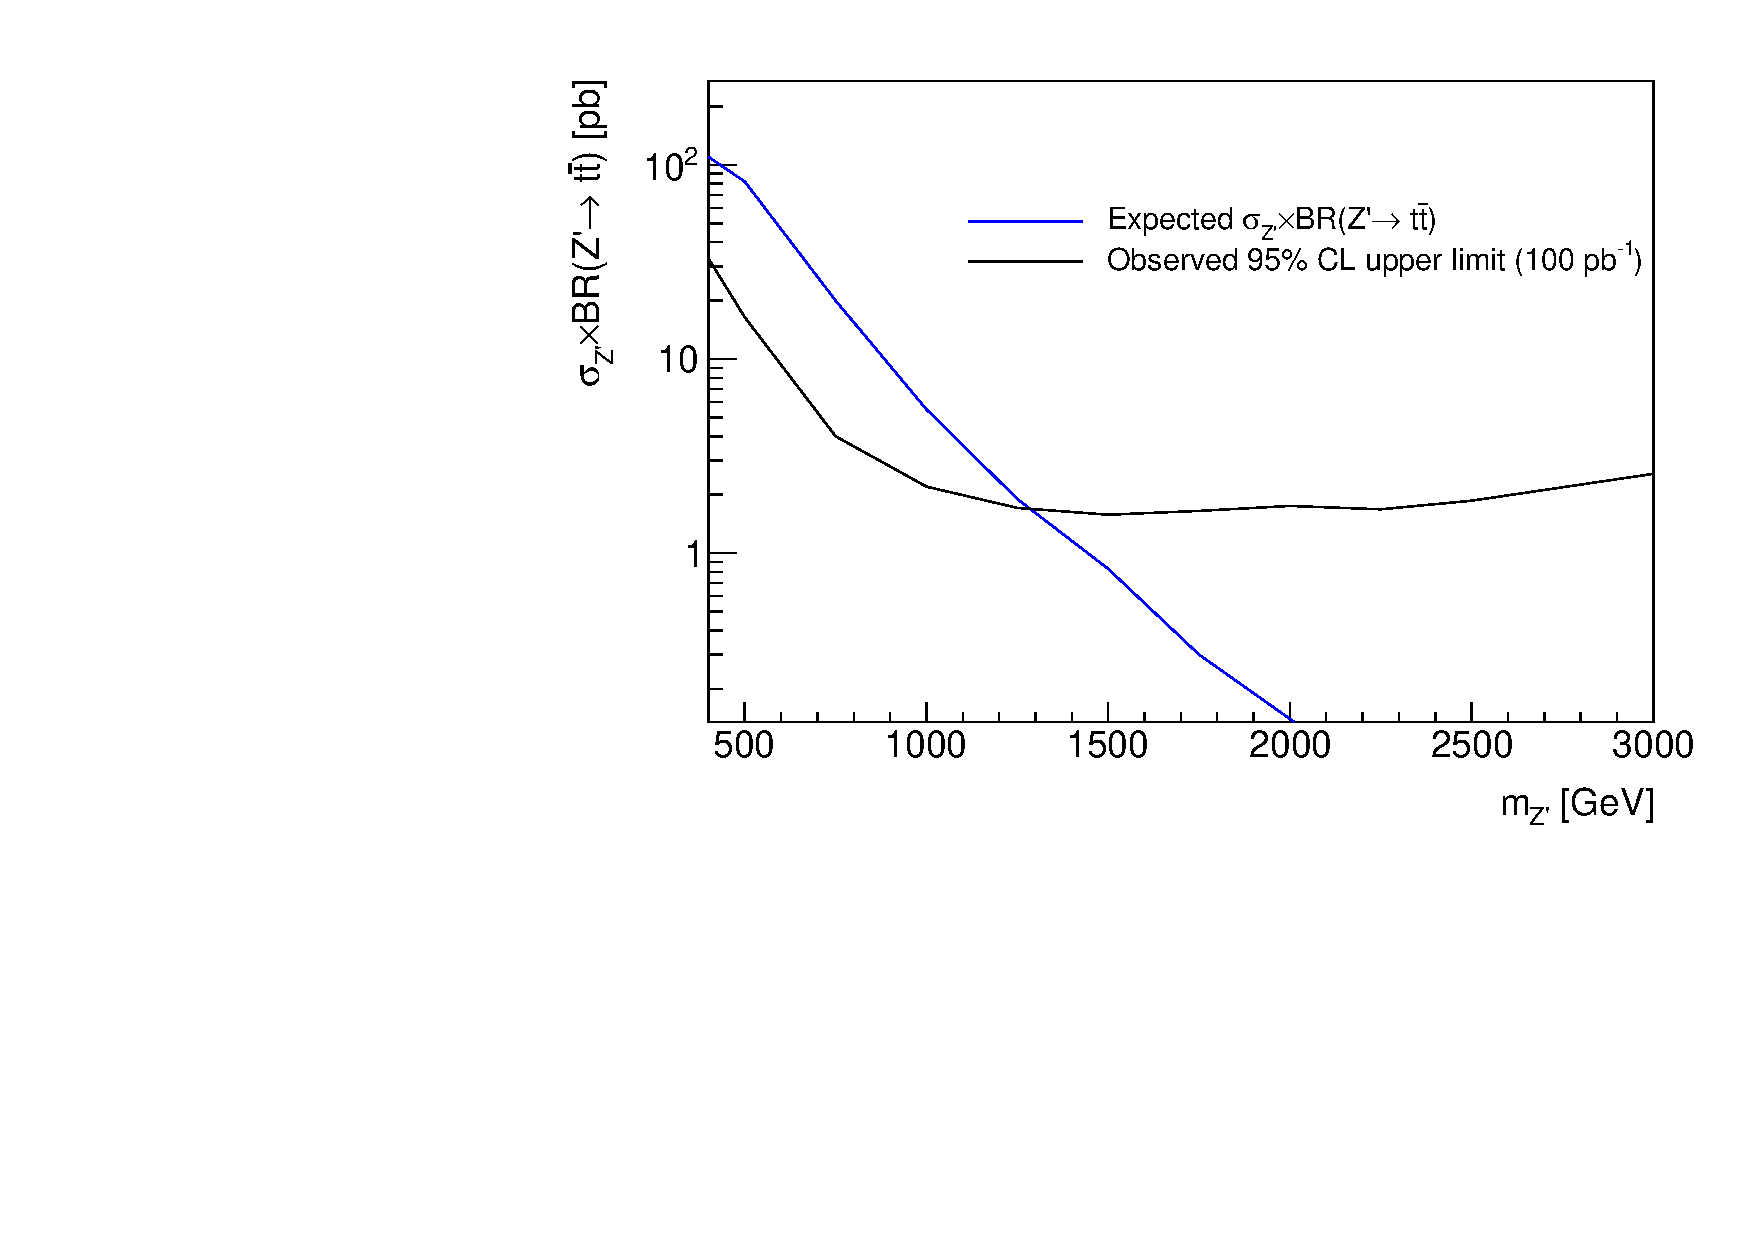
\includegraphics[width=\linewidth]{plots_and_txt/limits.pdf}
    \caption{Berechnete erwarteten oberen Ausschlussgrenzen der Wirkungsquerschnitte im $\SI{95}{\percent}$ Konfidenzintervall der unterschiedlichen $Z^\prime$-Massenhypothesen gegen ihre Masse. Zum Vergleich ist ebenfalls die erwartete Verteilung der Wirkungsquerschnitte dargestellt.}
    \label{fig:limit}
\end{figure}
